Historically, \textit{dxex} is based on \textit{PythonPDEVS}~\cite{PythonPDEVS}.
Python is a good language for prototypes, but performance has proven insufficient to compete with other simulation kernels~\cite{MasterThesis}.
\textit{Dxex} is a C++11-based \textsf{Parallel DEVS} simulator, based on the design of \textit{PythonPDEVS}.
Whereas the feature set is not too comparable, the architectural design, simulation algorithms, and optimizations, are highly similar.

We will not make a detailed comparison with \textit{PythonPDEVS} here, but only mention some supported features.
\textit{Dxex} supports, similarly to \textit{PythonPDEVS}, the following features: direct connection~\cite{SymbolicFlattening}, \textsf{Dynamic Structure DEVS}~\cite{DSDEVS}, termination conditions~\cite{JDF}, and a modular tracing and scheduling framework~\cite{PythonPDEVS}.
We do not elaborate on these features in this paper.
But whereas \textit{PythonPDEVS} only supports optimistic synchronization, \textit{dxex} support multiple synchronization protocols (though only in parallel).
This is in line with the design principle of \textit{PythonPDEVS}: allow users to pass performance hints to the simulation kernel.
In our case, a user can pass the simulation kernel the synchronization protocol to use for this model, or even switch the synchronization protocol during runtime.
Our implementation in C++11 also allows for optimizations which were plainly impossible in an interpreted language. \textit{Dxex} will use new optimizations from the C++14 standard when possible.

Since there is no universal \textsf{DEVS} model standard, \textit{dxex} models are incompatible with \textit{PythonPDEVS} and vice versa.
This is due to \textit{dxex} models being grafted on C++11, whereas \textit{PythonPDEVS} models are grafted on Python.

In the remainder of this section, we will elaborate on our prominent new feature: the efficient implementation of multiple synchronization protocols within the same simulation tool, which are offered transparently to the model.

\subsection{Synchronization protocols}
We previously explained the existence of different synchronization protocols, each optimized for a specific kind of model.
As no single synchronization protocol is ideal for all models, a general purpose simulation tool should support multiple protocols.
Currently, most parallel simulation tools choose only a single synchronization protocol due to the inherent differences between protocols.
We argue that a real general purpose simulation tool should support sequential, conservative, and optimistic synchronization, as is the case for \textit{dxex}.

These different protocols relate to three different model characteristics.
Conservative synchronization for when high lookahead exists between different nodes, and barely any blocking is necessary.
Optimistic synchronization for when lookahead is unpredictable, or there are rare (almost) instantaneous events.
Finally, sequential simulation is still required for models where parallelism is bad, where all protocols actually slow down simulation.

\subsubsection{Sequential}
Our sequential simulation algorithm is very similar to the one found in \textit{PythonPDEVS}, including many optimizations.
Minor modifications were made, though, such that it can be overloaded by different synchronization protocol implementations.
This way, the \textsf{DEVS} simulation algorithm is implemented once, but parts can be overridden as needed.
In theory, more synchronization protocols (\textit{e.g.}, other algorithms for conservative synchronization) can be added without altering our design.

An overview of \textit{dxex}'s design is given in Figure~\ref{fig:class_diagram}.
It shows that there is a simulation \texttt{Core}, which simulates the \texttt{AtomicModel}s connected to it.
The superclass \texttt{Core} represents the sequential simulation core.
Subclasses define specific variants, such as \texttt{ConservativeCore} (conservative synchronization), \texttt{OptimisticCore} (optimistic synchronization), and \texttt{DynamicCore} (\textsf{Dynamic Structure DEVS}).

\begin{figure*}
    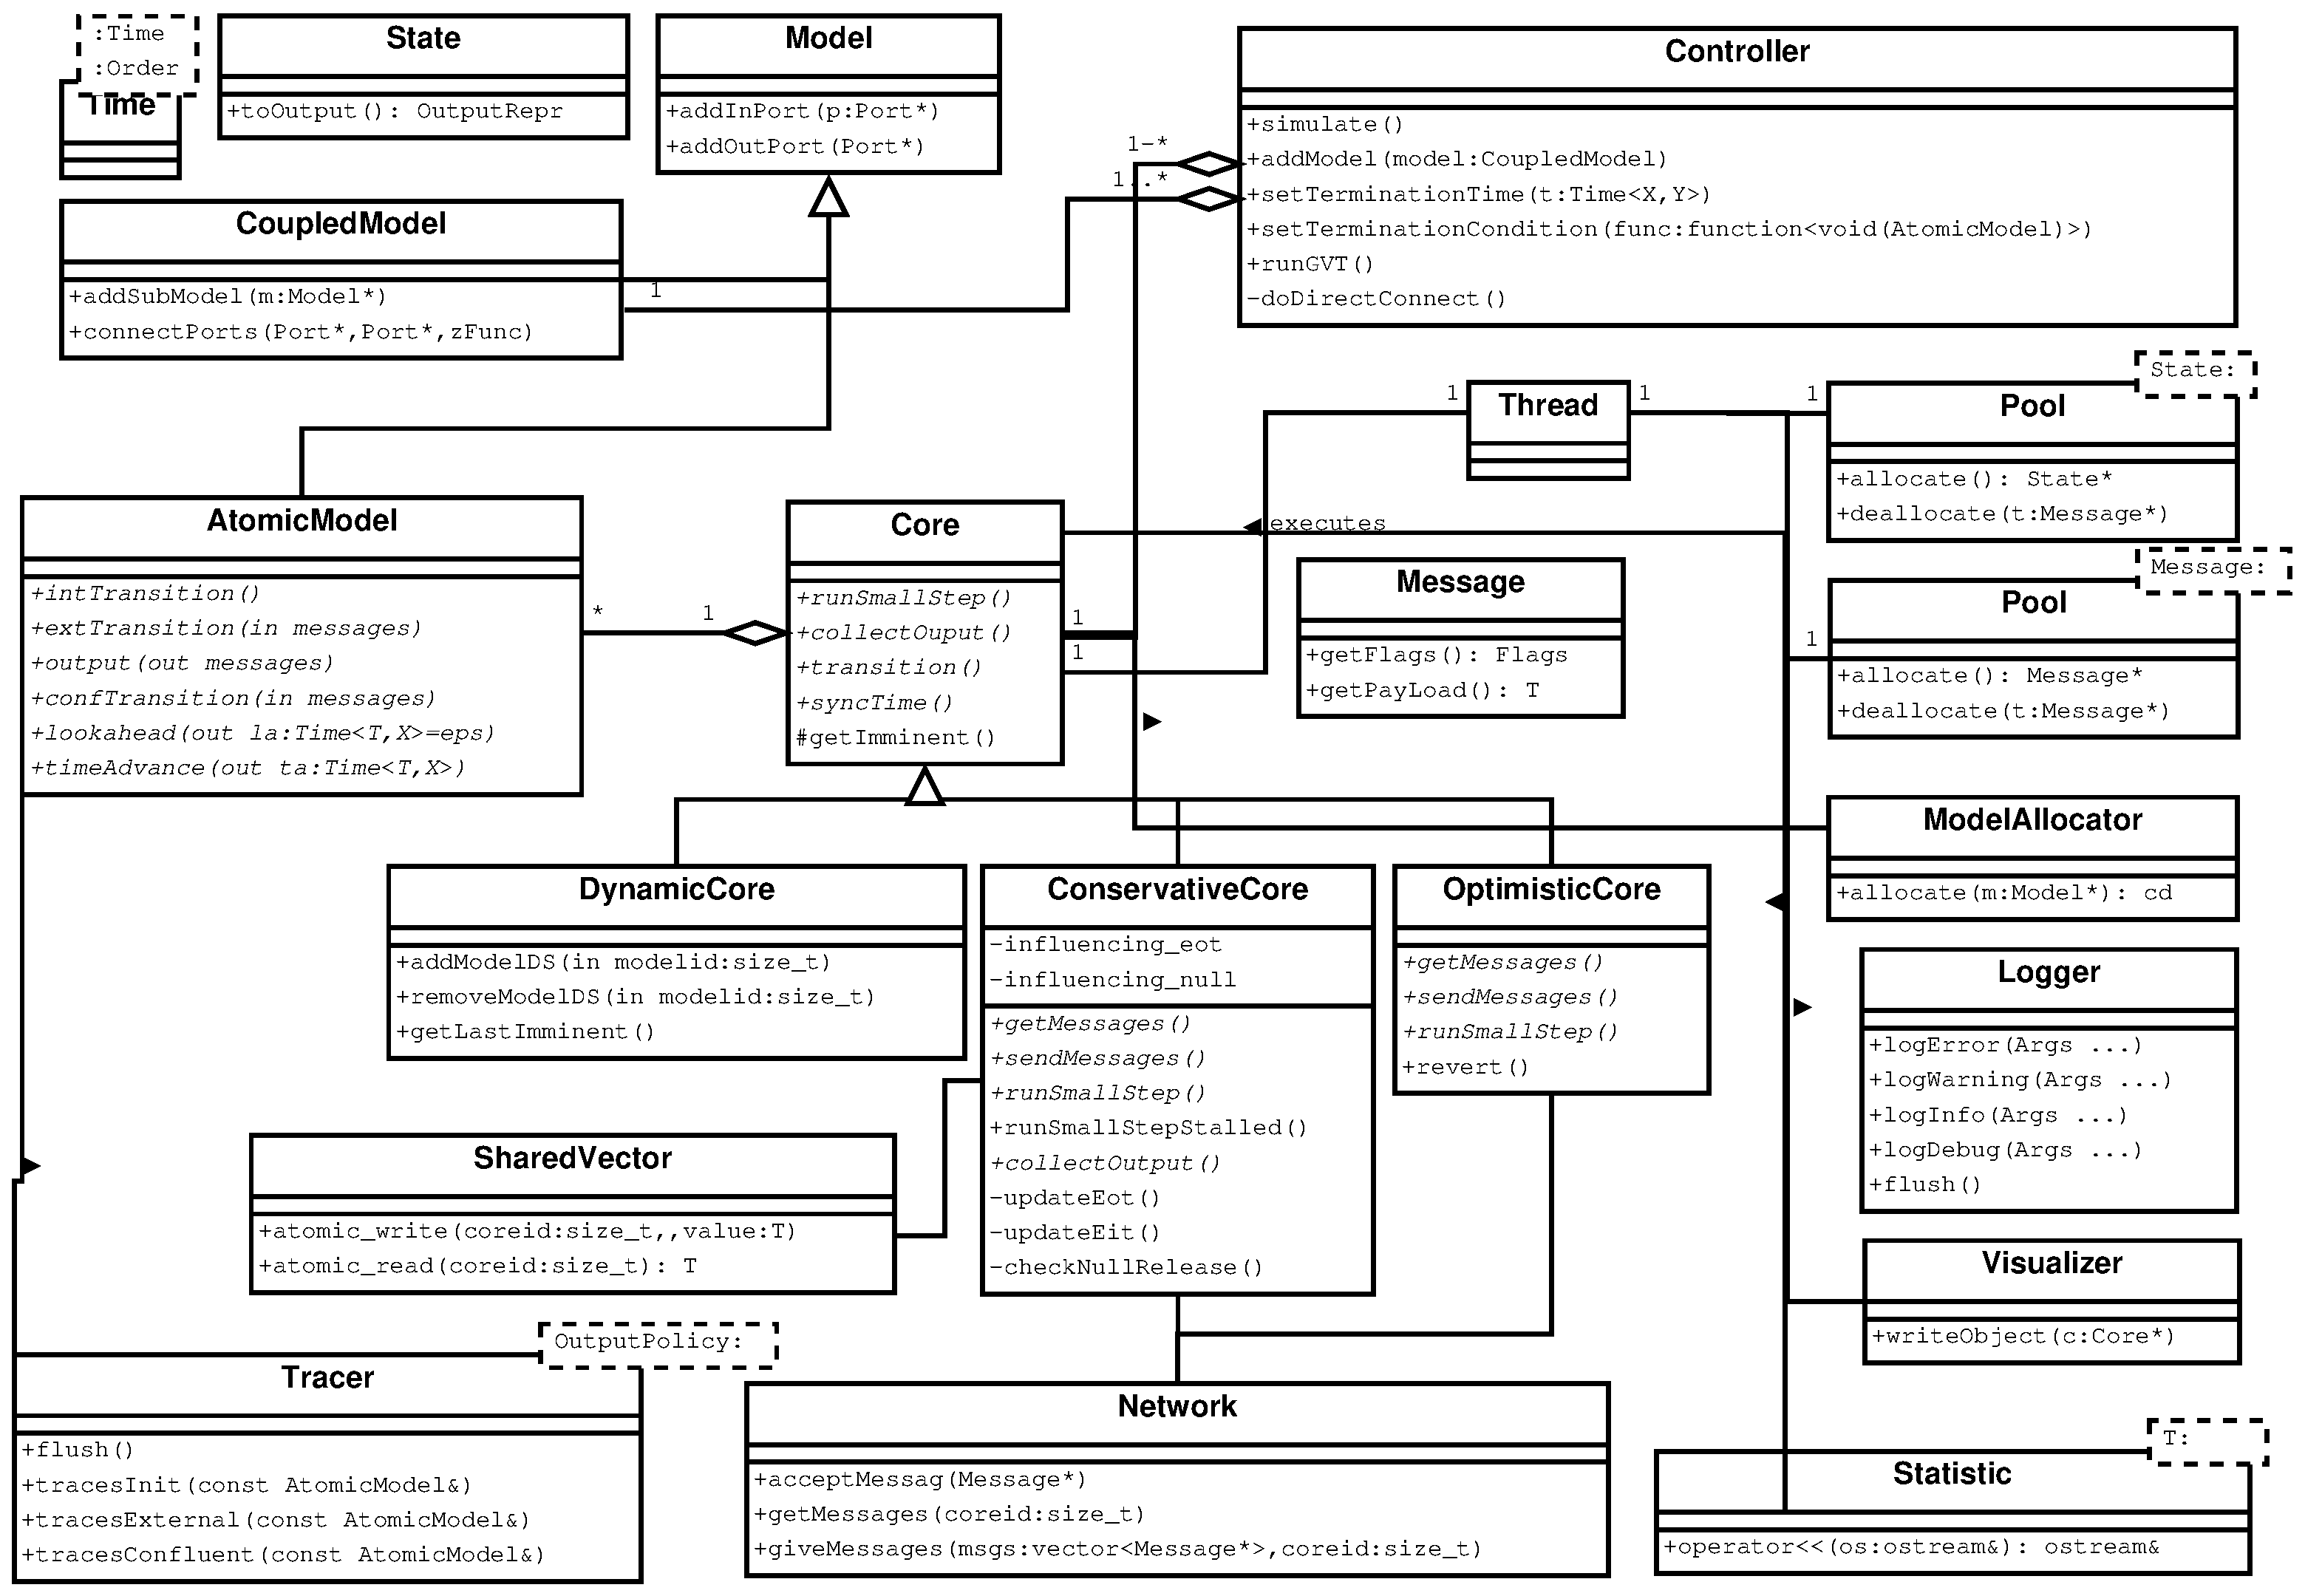
\includegraphics[width=\textwidth]{fig/cores_class_diagram.eps}
	\caption{\textit{Dxex} design.}
	\label{fig:class_diagram}
\end{figure*}

\subsubsection{Conservative}
For conservative synchronization, each node must determine the nodes it is influenced by.
Each model needs to provide a lookahead function, which determines the lookahead depending on the current simulation state.
Within the returned time interval, the model promises not to raise an event.
A node aggregates this information to compute its Earliest Output Time (EOT).
This value is communicated to other nodes through shared memory.

Reading and writing to shared memory is done through the use of the new C++11 synchronization primitives.
Whereas this was also possible in previous versions of the C++ standard, by falling back to non-portable C functions, it was not a part of the C++ language standard.
C++11 further allows us to make the implementation portable, as well as more efficient: the compiler makes further optimizations to heavily used components.

\subsubsection{Optimistic}
For optimistic synchronization, each node must be able to roll back to a previous point in time.
This is often implemented through the use of state saving.
This needs to be done carefully in order to avoid unnecessary copies, and minimize the overhead.
We use the default: explicitly save each and every intermediate state.
Mattern's algorithm~\cite{mattern} is used to determine the GVT, as it runs asynchronously and uses only $2n$ synchronization messages.
Once the GVT is found, all nodes are informed of the new value, after which fossil collection is performed, and irreversible actions are committed.

The main problem we encountered in our implementation is the aggressive use of memory.
Frequent memory allocation and deallocation caused significant overheads, certainly when multiple threads do so concurrently.
This made us switch to the use of thread-local %(using \textit{tcmalloc})% see page 6 for introducing tcmalloc
 memory pools.
Again, we made use of specific new features of C++11, that are not available in Python, or even previous versions of the C++ language standard.

\subsection{Synchronization Protocol Transparency}
We define synchronization protocol transparency as having a single model, which always can be executed on each supported synchronization kernel, without any modifications.
User should thus only provide one model, implemented in C++11, which can be simulated using sequential execution, conservative synchronization, or optimistic synchronization.
The synchronization protocol to use is a simple configuration option.
The exception is conservative synchronization, where a lookahead function is required, which is not used in other synchronization kernels.
Two options are possible: either a lookahead function must always be provided, even when it is not required and possibly not used, or we use a default lookahead function if none is defined.

Always defining a lookahead function might seem redundant, especially should the user never want to use conservative synchronization.
Defining the lookahead is difficult and can often be unpredictable.
The more attractive option is for the simulation tool to provide a default lookahead function, such that simulation can run anyway, but likely not at peak performance.
Depending on the model, simulation performance might still be faster than sequential simulation. 

Defining a lookahead function is therefore recommended in combination with conservative synchronization, but is not a necessity, as a default value $\epsilon$ (\textit{i.e.}, the smallest representable timestep) is used otherwise. Providing this default implementation has no impact in sequential or optimistic simulation, since the function is never called the compiler will optimize it out. By providing this default implementation in the model base class we ensure that a model can run in sequential, optimistic and conservative simulation by default.

\subsection{Increasing Parallelism}
The goal of our contribution is to increase simulation performance as much as possible, leveraging parallel computation in the process.
Parallelizing the simulation kernel goes further, however, than merely implementing the different synchronization protocols.

We observed that after implementing all synchronization protocols, performance was still not within acceptable levels.
Profiling revealed that most of the overhead was caused by two issues: memory management and random number generation.
For both, it is already known that they can have significantly impact on parallelizability of code, since they introduce sequential blocks.
Both were tackled using approaches that are in common use in the parallel programming world.
We briefly mention how the application of these techniques influences our performance.

\subsubsection{Memory Management}
\label{sec:4-subsec:overhead-pgraph:memory}
\begin{figure}
    \center
    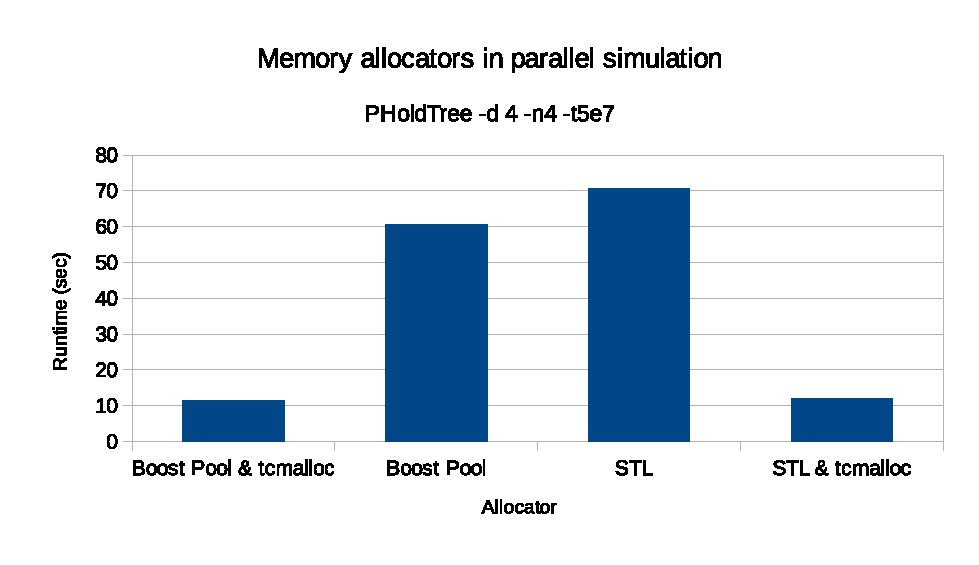
\includegraphics[width=\columnwidth]{fig/memory_allocators_parallel.eps}
    \caption{Effect of memory allocators on parallel execution time.}
    \label{fig:memallocators_parallel}
\end{figure}
Memory management is traditionally seen as one of the major bottlenecks in parallel computation~\cite{Memory}: memory bandwidth doesn't increase as fast as the number of cores using it.
While this is always a problem, it is aggravated in \textit{dxex} by providing automatic memory management for events and states.
A model written for sequential simulation will run correctly in a conservative or optimistic simulation without altering (from the point of view of the modeller) the (de)allocation semantics of events or states.

Furthermore, allocating and deallocating memory by making calls to the operating system, as is typically done by calls such as \texttt{malloc}, happens sequentially.
To counter this, our memory allocators are backed by a thread-aware pooling library.
In a sequential simulation kernel no allocated event persists beyond a single time advance, even allowing the use of an arena-style allocator.
Conservative and optimistic simulation need to use generic pool allocators since events are shared across kernels and thus have a different lifetime.

Intra-kernel events can be (de)allocated without requiring synchronization with the other kernels. 
They can be returned immediately to the memory allocator as the lifetime of these objects is known at creation.
In contrast inter-kernel events need a GVT algorithm to determine when safe deallocation can occur, even in conservative synchronization.
As a result simulations with many inter-kernel events suffer a performance hit, whereas the impact of many intra-kernel events can be minimized using arena ~\cite{Arena} allocators.

\textit{Dxex} uses \textit{Boost Pool}~\cite{boostpool} allocators in parallel simulation kernels and arena-style allocators for sequential simulation.
The latter can be faster, but at the cost of extra configuration.
The allocators are supplemented by the library \textit{tcmalloc}~\cite{tcmalloc}, which reduces lock contention in \texttt{malloc} calls.

We primarily investigate this for optimistic simulation, as this is the most memory consuming mode of simulation~\cite{FujimotoBook}.
Simulation execution times for all four combinations are shown in Figure~\ref{fig:memallocators_parallel}.
Optimistic simulation greatly benefits from the use of \textit{tcmalloc}, regardless of the allocator.
Nonetheless the pool allocator also reduces the allocation overhead, though only by a relatively small fraction.
Both techniques are required to reduce the overhead of memory allocations in \textit{dxex}, and are turned on by default.

Both pools and \textit{tcmalloc} try to keep memory allocated instead of returning it to the Operating System (OS).
As a result, the OS will usually report memory consumption that is higher than the actual amount of stored data.

\subsubsection{Random Number Generators}
Random Number Generators (RNG) are another aspect of the program that can limit parallelization.
All accesses to the RNG will result in the modification of a global (\textit{i.e.}, shared between threads) variable.
This easily becomes a bottleneck in simulation, since random numbers are a common occurence in simulation~\cite{Random}.
As such, a non-trivial amount of time in a simulation is often spent waiting for an RNG.

We of course still need to guarantee determinism and isolation between the calls to the RNG, as well as avoiding excessive synchronization.
\textit{Dxex} uses the Tina RNG collection (TRNG)~\cite{PhysRevE.75.066701} as an alternative random number generator with performance and multithreading in mind.
Since the RNG is an implicit part of the state in the \textsf{Parallel DEVS} formalism, though often not implemented as such, we evaluated performance for both approaches: one global RNG per thread, and one RNG per atomic \textsf{DEVS} model.

We see in Figure~\ref{fig:Queuerngspeedup} that storing the RNG in the state is very expensive for the default Standard Template Library (STL) random number generator.
This is primarily caused by the significant difference in size: 2504 bytes for the STL random number generator, and 24 bytes for the Tina random number generator.
\textit{Dxex}'s sequential and conservative kernels are insensitive to storing the RNG object in the atomic model state, since no copying/state saving occurs in \textit{dxex} conservative simulation.
The optimistic kernel is clearly affected, as it needs to copy more bytes in every transition due to state saving.

Figure~\ref{fig:Queuerngspeedup} shows that \textit{dxex} in sequential simulation is three times faster using TRNG compared to using the STL RNG.
For parallel simulation, the synchronization overhead seems to be the main bottleneck, as seen by the big speedup gap between sequential and parallel simulation.
Conservative synchronization is almost insensitive to the changing of the RNG, though a slight increase in performance can be noted.
Optimistic synchronization slows down significantly when the RNG becomes part of the model state, since the state needs to be copied as well.
This becomes a significant overhead when using the STL RNG, since performance plummets to a fraction of the original.
Using TRNG avoids this problem completely, as the size of the RNG state is negligible.

\begin{figure}
    \center
    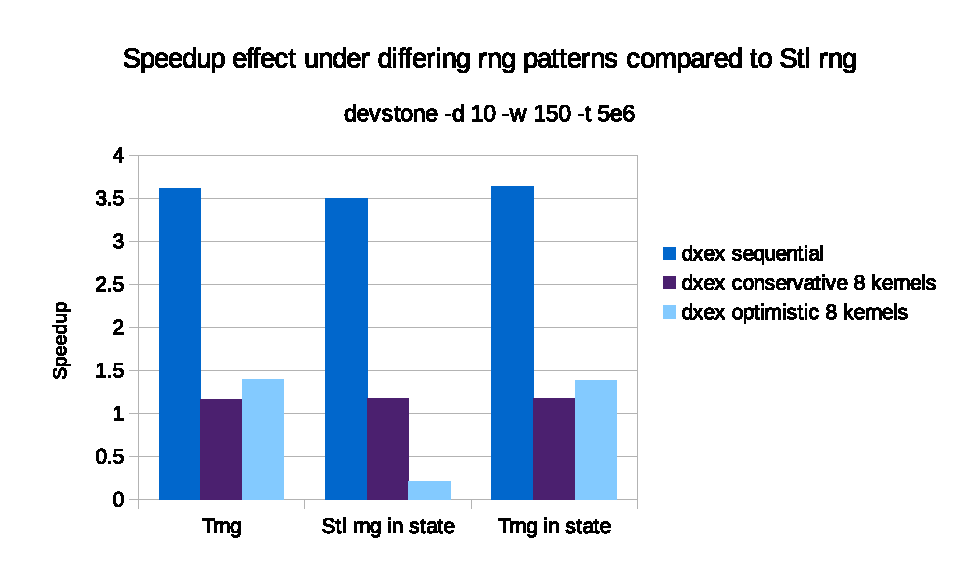
\includegraphics[width=\columnwidth]{fig/rngspeedupeffectdevstone.eps}
    \caption{Speedup with different RNG usage patterns compared to STL random number generator.}
    \label{fig:Queuerngspeedup}
\end{figure}
